% Szglab4
% ===========================================================================

\chapter{Követelmény, projekt, funkcionalitás}

\thispagestyle{fancy}

\section{Bevezetés}

\subsection{Cél}
\paragraph{Ezen dokumentum célja a Szoftver laboratórium 4. tárgy során meghírdetett csapatmunkában elkészítendő projekt kivitelezéséhez
szükséges követelmény, projekterv, funkcionális alapok megteremtése és rögzítése. A dokumentum tartalmazza a projekt során használt technológiák, eszközök
halmazát. Továbbá defininálja a szoftverrel és a fejlesztéssel kapcsolatos fogalmakat. Mindemellett lefekteti a szoftver legmagasabb architektúrális képét,
és megfogalmazza azon követelményeket, funkciókat, melyekenek a projekt során eleget kell tenni. Ezek priorizálása és a határidők meghatárzotása mind a dokumentum
felelőssége. Részletesen kitér a projekt realizálása során alkalmazott eljárásra, a csapat szinkronát biztosító elvekre, eszközökre.}

\subsection{Szakterület}
A projekt célja egy egyszerű számítógépes játék létrehozása a RUP fejlesztési módszer segítségével. A szoftvernek teljesítenie kell a Szoftver laboratórium IV. tárgy által adott specifikációban megfogalmazott követelményeket. \\ 
Az elkészült szoftver egy játékprogram, így nem egy hagyományos értelemben vett szakterület számára készül, hanem általános szórakoztatás céljából.

\subsection{Definíciók, rövidítések}

\begin{tabularx}{\textwidth}{| l | l |}
\hline
\textbf{Név} & \textbf{Definíció} \tabularnewline 
\hline\hline
\endhead
BME & Budapesti Műszaki Egyetem \tabularnewline \hline
Build system & olyan szoftverek együttese, amely automatizálja a szoftver \\
             & fordításának, tesztelésének, terjesztésének folyamatát \tabularnewline \hline
CI & Continuous Integration \\ 
   & folyamatos integráció; olyan fejlesztési folyamat, amely során \\
   & a fejlesztők a projekt kezdetétől fogva gyakori rendszerességel \\
   & összeillesztik és tesztelik kódjukat\tabularnewline \hline
Coverity & a projekthez használt statikus elemző \tabularnewline \hline
Git & Verziókezelő rendszer (VCS) \tabularnewline \hline
GitHub & A git verziókezelőt hostoló oldal (framework) \tabularnewline \hline
Gradle & a projekthez használt build system \tabularnewline \hline
Javadoc & egy olyan eszköz, amely a Java forráskódban \\ 
        & található kommentekből dokumentációt tud előállítani \tabularnewline \hline
JDK & Java Development Kit \tabularnewline \hline
JRE & Java Runtime Environment \tabularnewline \hline
LaTeX & A dokumentáció készítéséhez használt betűszedő rendszer \tabularnewline \hline
LGPL & GNU Lesser General Public License; \\ 
     & a projekt által használt nyílt forráskódú licenc \tabularnewline \hline
RUP & Ration Unified Process, egy szoftverfejlesztési módszer \tabularnewline \hline
Statikus elemzés & egy forráskódbázis elemzése lehetséges szoftverhibák \\
                  & megtalálása érdekében \tabularnewline \hline
Szoftlab 4 & Szoftver laboratórium 4. \tabularnewline \hline
TDD & Test-Driven-Development, tesztelésen alapuló szoftverfejlesztés \tabularnewline \hline
Travis CI & a projektben használt CI rendszer \tabularnewline \hline
UML & Unified Modeling Language \tabularnewline \hline
VCS & Version Control System, verziókezelő rendszer \tabularnewline \hline
\end{tabularx}


\subsection{Hivatkozások}
\begin{tabularx}{\textwidth}{| l | l |}
\hline
\textbf{Megnevezés} & \textbf{Link} \tabularnewline 
\hline\hline
\endhead
Szoftver Laboratórium 4. & iit.bme.hu/\textasciitilde szoftlab4 \tabularnewline \hline
Travis CI Docs & docs.travis-ci.com \tabularnewline \hline
GitHub & github.com \tabularnewline \hline
Waffle.IO & waffle.io  \tabularnewline \hline
LaTeX & latex-project.org \tabularnewline \hline
Coverity & coverity.com \tabularnewline \hline
Drone.IO & drone.io \tabularnewline \hline
Javadoc & oracle.com \tabularnewline \hline
Java & oracle.com \tabularnewline \hline
Visual Paradigm & visual-paradigm.com \tabularnewline \hline
Wikipedia & wikipedia.org \tabularnewline \hline
\end{tabularx}


\subsection{Összefoglalás}
\paragraph{
    A továbbiakban a dokumentum alapozva a fentebb megismert fogalmak definíciójára végigveszi a dokumentum céljában
    említett pontokat. Részletesen foglalkozik a megvalósítandó funkciókkal, definiálja a feltárt use-caseket majd végül
    napló formájában összegzi a csapat munkáját, a feladatokra fordított erőforrásokat. A projektterv során részletesen kitér
    a csapat által használt elvekre, eszközökre melyekkel a projekt sikeres leszállítását szándékoznak elérni. 
}

\section{Áttekintés}

\subsection{Általános áttekintés}
%\comment{A kialakítandó szoftver legmagasabb szintű architekturális képe. A fontosabb alrendszerek felsorolása, a közöttük kialakítandó interfészek lényege, a felhasználói kapcsolatok alapja. Esetleges hálózati és adattárolási elvárások.}

\indent A kialakítandó szoftver alapvetően egy játékprogram \emph{(továbbiakban: játék)}. Több rendszerre és alrendszerre is szükségünk van ahhoz, hogy a felhasználóval \emph{(továbbiakban: játékos)} a kapcsolatot tartsuk és számára a megfelelő játékélményt prezentáljuk.\\
\indent Három alapvető működési egységgel rendelkezik majd a program. Ezek pedig a következő funkciókat ellátó alrendszerek:
\begin{enumerate}
	\setlength\itemsep{0pt}
	\item A játékostól a játék irányába vett interakció
	\item A játéktól a játékos felé történő visszajelzés 
	\item A játék logikájának és állapotának kezelése
\end{enumerate}
Ezen rendszerek között kialakítandó interfészeket úgy kell megvalósítani, hogy azok biztosítsák a játékos számára az alkalmazásnak a gördülékeny működését. Ebből a felhasználónak prezentált kezelőfelületekkel az első két alrendszer rendelkezik.\\
\indent A programnak feltétlen szüksége lesz adattárolási lehetőségre, hogy a a játékos kérésére a játék állását el lehessen tárolni, és azt későbbi továbbjátszás céljából vissza állítható legyen.

\newpage
\subsection{Funkciók}
\paragraph{
Ezen pont a megrendelő által adott játékprogram funkcionális szempontból történő leírását tartalmazza, melyben részletesen kitér és tisztázza az elkészítendő termék funkcióit. Kiemelt célja a szekciónak, hogy szabatosan, tényszerűen fogalmazva biztosítsa, hogy megismerése után a dokumentum olvasójának ne legyen kétsége mit fog kapni a projekt leszállításakor. Felépítését tekintve törekedtünk, hogy a leírás során minden egyes megrendelő által adott követelményt a csapattól származó kiegészítő, egyértelműsítő funkciók kövessenek, ezzel növelve az egyértelműséget.
\\
A feladat leírásában elsősoron a játék legmagasabb váza jelenik meg, mely nevezhető a játék "alaphelyzetének" leírásaként. A játékos egy robotot irányít egy előre elkészített versenypályán, mely ugrálással tud mezőről mezőre pozíciót változtatni. Ebből a követelményből fakad, hogy a csapat körökre osztott játékmenetet képzel el, melynek során játékosról játékosra lehetőség nyílik a robotunkkal történő interakcióra. Minden játékos saját robottal rendelkezik, így szintén csapatunk közös döntése, hogy a játékban résztvevő személyek száma legalább kettő, de a játékmenet tempósságának és ezzel élvezhetőségének, izgalmának megtartása érdekében nem haladhatja meg a négyet. A megrendelő specifikiációjában szerepel, hogy a játék során a versenyben idő-komponens is létezik, ugyanakkor nem definiálja ezt milyen módon képzeli el. Csapatunk úgy gondolta, hogy a játékosok számára biztosít előre meghatározott időkereteket. A konzisztencia és izgalom érdekében nem enged tetszőleges időlimitet beállítani, hanem egy bő halmazból enged időkorlátokat választani, melyek szintén növelhetik a játék nehézségét, ugyanakkor kezdő játékosok számára lehetőség nyílik könnyedségre is. A másik talán legfontosabb játékdimenzió maga a tér, pálya, ahol a verseny játszódik. Ezen játékteret, hogy az időkorlát értelmet nyerjen a verseny során, a csapatunk huroknak képzelte el, mely lehetőséget ad változatos, ugyanakkor "végtelen" ideig játsztható versenyre. A pálya a játék indulásakor generálódik, véletlenszerű kanyarokkal, egyenesekkel, de garantáltan mindig hurkot alkot. A megrendelő által adott leírásban definiálja igényét, mely szerint a pályáról leeső robotok kiesnek a játékból, ez a hurok formájú pálya és a kanyarok miatt reális veszéllyé teszi ezt az eshetőséget. Az eddigiekben a játék általános képéről beszéltünk, most szeretnénk kitérni részeltesebben a játék menetére. A leírásból adott, hogy a robotok álló helyzetből indulnak kezdőpozíciójukból.
\\
Innentől kezdetét veszi az általunk elképzelt körökre osztott játék, melynek során a játékosonak lehetősége adódik minden körben a leírásban meghatározott sebességvektor egységnyivel történő módosításására, egy előre meghatázotott intervallumban. Ettől a sebességvektortól függően a játékosok minden körben lehetőséget kapnak ezen vektor által meghatározott arányos távolságra ugrani. A sebességvektor definíciója a fizikából adott, ugyanakkor esetünkben ennek módosítása diszkrét módon lehetséges. Triviálisan adott, hogy a nulla mértékű sebességvektor nem okoz elmozdulást a pályán, innentől pedig az egységnyivel növel értékek arányosan növelik az átugrott mezők számát. Irányát tekintve a 8 fél-égtáj felé mutathat, mellyel a játék nehézségét szeretnék növelni, hiszen így a kanyarok miatt jobban kell előre terveznie a játékosnak. Ezt a döntést nehezíti a pályán található, a megrendelő által kért, foltok, melyek hatással vannak a robotokra. A foltok jelenleg kétfélék lehetnek, mely szintén a megrendelő kérése, olajfoltok és ragacsfoltok. Előbbi a robotot, ezáltal a játékost képtelenné teszik a sebességvektor módosítására az adott körben. Utóbbira érzekve pedig a játékos sebessége megfeleződik. 
\\
Csapatunk fontosnak tartotta, hogy a körkörös pályából fakadóan a foltok eltűnnek, miután kiváltották hatásukat valamely robotra. Az előbb említett foltokból a robotoknak készletük van, melyet használhatnak nyerési esélyeik növelése érdekében, úgy hogy maguk mögött hagyják a játékos parancsára. Ezen készleteknek mennyiségük van, melyből a játék kezdetekor kapnak a robotok. Pótolni a felhasznált foltokat a pályán megjelenő dobozokból van lehetősége a játékosnak, melyekben véletlenszerűen találhatóak készletek, véletlenszerű mennyiségben. Ezzel a funckióval a játék izgalmát, a dobozokért történő versenyt, illetve a játékosok interakciójának növelését szeretnénk elérni. A foltok és dobozok a pályán az idő múlásával újratermelődnek, ezzel biztosítva a kiegyensúlyozott játékot. A dobozok felvételéhez a játékosoknak rá kell ugrani arra a mezőre, melyen egy doboz tartózkodik. A foltokhoz hasonlóan a doboz eltűnik a mezőről, ha ráugrottak és a benne található készlet bekerül a robot tárolójába. Fontosnak tartjuk kiemelni, hogy a készlet, melyet a játékos a dobozból nyer nem opcionális, azt kötelező elfogadnia. Ebből következik, hogy a készletek mennyiségére nem tettünk megkötés, egy robot bármennyit összegyűjthet, ezáltal növelve nyerési esélyeit a többivel szemben.
\\
A győzelem definiálása a leírásból adott, mely szerint a fentebb meghatározott időkomponens és az út függvényéből generált pontszám alapján dől el, hogy ki nyeri a versenyt. A megadott idő alatt a leghosszabb utat megtevő játékos nyer. Adott a kérdés, hogy hogyan definiáljuk az utat, hogy elkerüljük azt az eshetőséget, hogy a robot oda-vissza ugrál két mező között. A csapat erre megoldásnak azt találta ki, hogy a hurok alakú pályán egy vonalból induló robotoknak előre meghatározott haladási iránya van, mely nem kötelező, ugyanakkor csak ebben a (tangenciális) irányban történő elmozdulásból fakadó út számít a pontokba. A pályán a játékosok így haladnak körbe a hurkon, és idejük lejártával nincs lehetőségük újabb lépésekre. A játék akkor ér véget, amikor mindegyik játékos ideje lejár. Ekkor a legtöbbet "helyes" irányba ugrott robot tulajdonosa lesz a győztes. Ebből a funckióból fakad, hogy amennyiben valakinek lejárt az ideje még mindig lehet győztes, amennyiben a többiek a maradék idejükben nem tudnak felzárkózni hozzá útjukat tekintve. 
\\
A szekcióban fentebb említett funkciók szedete megtalálható lentebb táblázatos formában, mely már nem ennyire részletesen, inkább cím szinten sorolja fel a megvalósítandó és bevállalt jellemvonásokat. Továbbá a funckió előíróján, ötletgazdáján túl annak prioritását is taglalja. 
}

\subsection{Felhasználók}
A felhasználóknak legyen ismeretük PC-k (personal computer) alapvető kezelésében Windows operációs rendszeren és mind fizikailag mind mentálisan képesek legyenek billentyűzet és egér használatára.


\subsection{Korlátozások}
A szoftverre vonatkozó egyetlen előírás, hogy a HSZK gépein telepített Java könyvtárkészletet használja, ezzel biztosítva az ezen gépeken való megfelelő futást.

\subsection{Feltételezések, kapcsolatok}

\begin{tabularx}{\textwidth}{| l | l |}
\hline
\textbf{Megnevezés} & \textbf{Link} \tabularnewline 
\hline\hline
\endhead
Szoftver Laboratórium 4. & iit.bme.hu/\textasciitilde szoftlab4 \tabularnewline \hline
Java & oracle.com \tabularnewline \hline
Wikipedia & wikipedia.org \tabularnewline \hline
\end{tabularx}

\section{Követelmények}
\subsection{Funkcionális követelmények}

% Azonosító, Leírás, Ellenőrzés, Prioritás, Forrás, Use-case, Komment
\begin{tabularx}{\linewidth}{| l | X | l | l | l | m{1.9cm} | l |}
\hline
\textbf{Azonosító} & \textbf{Leírás} & \textbf{Ellenőrzés} & \textbf{Prioritás} & \textbf{Forrás} & \textbf{Use-case} & \textbf{Komment} \tabularnewline
\hline\hline
\endhead
F001 & Robotok egy előre elkészített versenypályán ugrálnak & bemuatás & alapvető & megrendelő & Ugrás &  \tabularnewline \hline
F002 & A Játékosok egymás után kerülnek körönként sorra & bemutatás & alapvető & csapat & & \tabularnewline \hline
F003 & Az időt Játékosonként tarjuk nyilván. Akkor ér véget ha az utolsó Játékosnak is elfogy az ideje. Ha valakinek elfogyott akkor többet nem ugorhat. & bemutatás & alapvető & csapat & & \tabularnewline \hline
F004 & Előre megadott időkorlátokból lehet választani & bemutatás & alapvető & csapat & & \tabularnewline \hline
F005 & A játékot egyszerre minumum 2, maximum 4 Játékos játszhatja & bemutatás & alapvető & csapat & & \tabularnewline \hline
F006 & A pálya versenypálya szerű azaz hurkot alkot, játékmenet indulásakor generálódik véletlenszerű kanyarokkal & bemutatás & fontos & csapat & & \tabularnewline \hline
F007 & A pályáról leugró robotok elakadnak, kiesnek a játékból & bemutatás & alapvető & megrendelő & Elakaszt &  \tabularnewline \hline
F008 & Robotok álló helyzetből és kezdőpozíciójukról indulnak & bemutatás & alapvető & megrendelő &  &  \tabularnewline \hline
F009 & Robotok körönként egy egységhosszú sebességvektorral változtathatják a sebességüket egy megadott maximális nagyságig & bemutatás & alapvető & megrendelő & Sebesség\-vektort változtat &  \tabularnewline \hline
F010 & Robotok körönként ugorhatnak a megadott sebességvektorukkal arányos távolságra & bemutatás & alapvető & megrendelő & Ugrás &  \tabularnewline \hline
F011 & A pályán lehetnek különböző foltok melyek hatással vannak a rajtuk áthaladó Robotokra & bemutatás & alapvető & megrendelő & Támad &  \tabularnewline \hline
F012 & Vannak olajfoltok melyekre érkezve sebesség módosítására nincsen mód & bemutatás & alapvető & megrendelő & Olajfoltot hagy & \tabularnewline \hline
F013 & Vannak ragacsfoltok melyekre érkezve a sebesség megfeleződik & bemutatás & alapvető & megrendelő & Ragacsfoltot hagy & \tabularnewline \hline
F014 & Ha egy Robot megérkezik a foltra akkor miután kifejtette hatását eltűnik & bemutatás & opcionális & csapat & & \tabularnewline \hline
F015 & A Robotok fel vannak szerelve foltkészlettel, amelyeket a játékos parancsára maguk mögött tudnak hagyni. & bemutatás & alapvető & megrendelő & Támad & \tabularnewline \hline
F016 & A pályán véletlenszerűen elhelyezett elemek vannak, melyeket a Robotok felvéve további foltokhoz juthatnak & bemutatás & opcionális & csapat & & \tabularnewline \hline
F017 & Győztes az a játékos aki a megadott idő alatt a leghosszabb utat tudja megtenni & kiértékelés & alapvető & megrendelő & & \tabularnewline \hline
\end{tabularx}

\subsection{Erőforrásokkal kapcsolatos követelmények}

% Azonosító, Leírás, Ellenőrzés, Prioritás, Forrás, Komment
\begin{tabularx}{\linewidth}{| l | X | l | l | l | X |}
\hline
\textbf{Azonosító}   & \textbf{Leírás} & \textbf{Ellenőrzés} & \textbf{Prioritás} & \textbf{Forrás} & \textbf{Komment} \tabularnewline
\hline\hline
\endhead
E001 & JRE 6 vagy újabb & bemutatás & alapvető & megrendelő &  \tabularnewline \hline
E002 & JRE-hez szükséges minimális rendszerkövetelményekkel rendelkező számítógép & bemutatás & alapvető & megrendelő & \tabularnewline \hline
E003 & Alapvető perifériák & bemutatás & alapvető & megrendelő & monitor, egér, billentyűzet \tabularnewline \hline
E004 & Git & nincs & alapvető & csapat & verziókezelő \tabularnewline \hline
E005 & GitHub & nincs & alapvető & csapat & account minden csapattag részére  \tabularnewline \hline
E006 & TravisCI & nincs & alapvető & csapat & continous integration \tabularnewline \hline
E007 & Coverity & nincs & alapvető & csapat & statikus ellenörző \tabularnewline \hline
E008 & Waffle.io & nincs & opcionális & csapat & projekt management \tabularnewline \hline
E009 & JDK 6 vagy újabb & nincs & alapvető & csapat & \tabularnewline \hline
E010 & Gradle & nincs & alapvető & csapat & build rendszer  \tabularnewline \hline
E011 & Vim & nincs & opcionális & csapat & szövegszerkesztő \tabularnewline \hline 
E012 & GEdit & nincs & opcionális & csapat & szövegszerkesztő \tabularnewline \hline
E013 & Eclipse & nincs & opcionális & csapat & IDE \tabularnewline \hline
E014 & IntelliJ IDEA & nincs & opcionális & csapat & IDE \tabularnewline \hline
E015 & LaTeX & nincs & alapvető & csapat & dokumentáció készítéséhez \tabularnewline \hline
E016 & TeXStudio & nincs & opcionális & csapat & LaTeX IDE \tabularnewline \hline
E017 & Visual Paradigm & nincs & alapvető & csapat & UML IDE \tabularnewline
\hline
\end{tabularx}

\subsection{Átadással kapcsolatos követelmények}

% Azonosító, Leírás, Ellenőrzés, Prioritás, Forrás, Komment
\begin{tabularx}{\linewidth}{| l | X | l | l | l | X |}
\hline
\textbf{Azonosító}   & \textbf{Leírás} & \textbf{Ellenőrzés} & \textbf{Prioritás} & \textbf{Forrás} & \textbf{Komment} \tabularnewline
\hline\hline
\endhead
A001 & Dokumentáció beadás & bemutatás & alapvető & megrendelő & heti rendszerességel, hétfőnként \tabularnewline \hline
A002 & Szkeleton beadás & beadás & alapvető & megrendelő & márc. 23., beadórendszerben \tabularnewline \hline
A003 & Szkeleton bemutatás & bemutatás & alapvető & megrendelő & márc. 25. \tabularnewline \hline
A004 & Prototípus beadás & beadás & alapvető & megrendelő & ápr. 20., beadórendszerben \tabularnewline \hline
A005 & Prototípus bemutatás & bemutatás & alapvető & megrendelő & ápr. 22.  \tabularnewline \hline
A006 & Grafikus változat beadás & beadás & alapvető & megrendelő & máj. 11., beadórendszerben  \tabularnewline \hline
A007 & Grafikus változat bemutatás & bemutatás & alapvető & megrendelő & máj. 13. \tabularnewline \hline
A008 & A program fut a laboratóriumban kijelölt számítógépeken & bemutatás & alapvető & megrendelő & \tabularnewline \hline
A009 & A program telepíthető külső segítség nélkül & bemutatás & fontos & megrendelő & \tabularnewline \hline
A010 & JRE 1.6 vagy újabb meglétének ellenőrzése & kiértékelés & alapvető & csapat & telepítés, ha nem található \tabularnewline \hline
\end{tabularx}

\subsection{Egyéb nem funkcionális követelmények}

% Azonosító, Leírás, Ellenőrzés, Prioritás, Forrás, Komment
\begin{tabularx}{\linewidth}{| l | X | l | l | l | X |}
\hline
\textbf{Azonosító}   & \textbf{Leírás} & \textbf{Ellenőrzés} & \textbf{Prioritás} & \textbf{Forrás} & \textbf{Komment} \tabularnewline
\hline\hline
\endhead
NF001 & A programnak legyen magyar nyelvű kezelőfelülete. & egyértelmű & alapvető & megrendelő & \tabularnewline \hline
NF002 & Legyen mód a megfogalmazott követelmények tesztelésére. & tesztesetek & fontos & megrendelő & \tabularnewline \hline
NF003 & Legyenek unit-tesztek. & tesztesetek & alapvető & fejlesztő &  \tabularnewline \hline
NF004 & Egy felhasználó által kiadott parancs után a program vagy az operációs rendszer 1 másodpercen belül biztosítson valamilyen választ a felhasználó számára.  & mérés, tesztelés & alapvető & megrendelő & Legalább a következő teljesítménnyel rendelkező PC-k esetében: Core i7 3610QM, 8GB RAM \tabularnewline \hline

	
\end{tabularx}


\section{Lényeges use-case-ek}
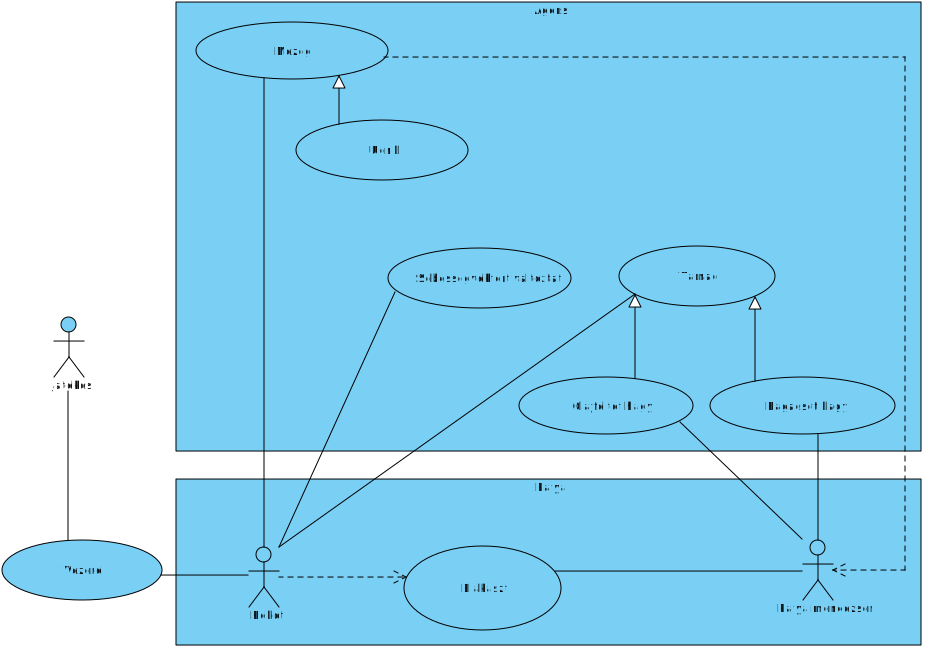
\includegraphics[width=\textwidth]{./chapters/chapter02/importantUseCases_c.pdf}

\subsection{Use-case leírások}

\usecase{Vezérel}%
{Játékos ezen a módon tudja irányítani a Robotot a pályán}%
{Játékos; Robot}%
{Játékos a helyzet alapján dönt arról, hogy a Robotnak mit kéne lépnie és utasítani fogja arra, hogy ezt tegye is meg}

\usecase{Mozog}%
{A Robot mozoghat a pályán. A mozgásnak magának több módja is van}
{Robot}
{A Játékos irányítja a Robotot annak érdekében, hogy közelebb kerülhessen a célhoz. Ehhez természetesen mozognia kell}

\usecase{Ugrik}%
{Mozgás egy fajtája, amely a sebességgel arányos lépést tesz}%
{-}%
{A Játékos a Robotot a cél felé irányítása folyamán ugrásra utasítja}

\usecase{Sebességvektort változtat}%
{A Robot megváltoztathatja a sebességvektorát}%
{Robot}%
{A Játékos a Robot cél fele való vezérélésének folytán megváltoztathatja a sebesség irányát és nagyságát is, például a pályán lévő kanyar bevételének céjából}

\usecase{Támad}%
{A Robot valamiképpen támadást végezhet a pályán}%
{Robot}%
{Ilyen támadásokkal más Robotokat hátráltathat valamilyen módon a továbbhaladásban}

\usecase{Olajfoltot hagy}%
{Egy Támadás fajta}%
{Pálya menedzser}%
{Robotok egymás hátráltatására olajfoltot hagyhatnak a pályán, mely ezután akadályozza a további Robotokat a sebesség megváltoztatásában}

\usecase{Ragacsot hagy}%
{Egy Támadás fajta}%
{Pálya menedzser}%
{Robotok egymás hátráltatására ragacsfoltot hagyhatnak a pályán, mely ezután megfelezi a többi Robotnak a sebességvektorát}

\usecase{Elakaszt}%
{Robotok szabálybetartásának végrehajtása}%
{Pálya menedzser}%
{Egy olyan Robot meg megsértette a játék szabályait valamely módon például lemegy a pálya határairól, azt a Pálya menedzser elakaszhatja ezáltal kizárva a játékból}

\section{Szótár}

\begin{tabularx}{\textwidth}{| l | l |}
\hline
\textbf{Bejegyzés} & \textbf{Definíció} \tabularnewline 
\hline\hline
\endhead
    ágens & a robot maga \tabularnewline \hline
    ágensleíró &  az állapotot meghatározó változó, melyből több is lehet, ezeket a telepes változtathatja \tabularnewline \hline
    áll &  robot kezdeti állapota, jelenlegi helyzetben a sebességvektor 0 mértékű \tabularnewline \hline
    állapot &  a robot leírója, mely meghatározza az érvényes cselekvéseinek halmazát \tabularnewline \hline
    buff &  olyan hatás, mely pozitív vagy negatív módon járulhat hozzá a robot játékához \tabularnewline \hline
    birtokol & a robot tárolójában készlet van belőle \tabularnewline \hline
    célfüggvény & a győzelemhez ennek maximalizálása szükséges, a pontszám növelése  \tabularnewline \hline
    doboz & olyan objektum a pályán, melyre lépre a robot véletlenszerűen kap valamilyen készletet\tabularnewline \hline
    entitás &  egy szereplő a játékban \tabularnewline \hline 
    esemény & valamely történés, melyet egy játékos cselekvése váltott ki \tabularnewline \hline
    folt &  a mezőn helyezkedik el, buffot válthat ki \tabularnewline \hline
    grid (négyzetrács) & a pálya felosztása, jelenleg négyzetesen \tabularnewline \hline
    győztes &  jelenleg a leghosszabb utat megtett robot \tabularnewline \hline
    használ &  a készlet egy elemét aktiválja, mely kiváltja az általa definiált buffot \tabularnewline \hline
    határ &  a pálya tulajdonsága, melyen túl nincsenek mezők \tabularnewline \hline
    idő &  a verseny időtartama \tabularnewline \hline
    irányít &  a folyamat melynek során a telepes a robot ágensleíróit módosíthatja \tabularnewline \hline
    játékos &  a telepest irányító entitás \tabularnewline \hline
    készlet &  egy adott tárgy leírására alkalmas, mennyiséggel rendelkezik, a robot használhatja \tabularnewline \hline
    kiesik &  a robot elhagyja a pályát \tabularnewline \hline
    kivált &  esemény, melynek során valamely entitásra hat a kiváltó objektum \tabularnewline \hline
    mező &  objektum vagy objektumok tárolására alkalmas egység, lehet szabad és foglalt \tabularnewline \hline
    mozog &  a robot pozícióját megváltoztató vezérlés \tabularnewline \hline
    nyerési feltételek &  azon feltételek, melyeket egy robot teljesítve győztesnek tekinthető \tabularnewline \hline
    objektum &  jelenleg robot, folt \tabularnewline \hline
    olajfolt &  egy folt, mely kivált egy buffot, ami nem engedi a sebességvektor megváltoztatását \tabularnewline \hline
    olajkészlet &  egy készlet, mely az olajfolttal egyező buffot vált ki \tabularnewline \hline
    pálya &  a játéktér, mely mezőkből áll \tabularnewline \hline
    perk (áldás) & olyan buff melynek a robotra pozitív hatása van, növeli a nyerési esélyeket  \tabularnewline \hline
    pontszám &  a győztes meghatározásához szükséges mérték, a megtett útban \tabularnewline \hline
    pozíció &  a robot helyzete a pályán \tabularnewline \hline
    ragacsfolt &  egy folt, mely kivált egy buffot, ami megfelezi a sebességvektort \tabularnewline \hline
    ragacskészlet &  egy készlet, mely a ragacsfolttal egyező buffot vált ki \tabularnewline \hline
    robot &  a pályán elhelyezkedő, mezőn álló entitás, melyet a telepes irányít \tabularnewline \hline
    sebesség &  a robot mozgását meghatározó mérték, megmondja a robot hány mezőt léphet \tabularnewline \hline
    sebességvektor &  egy ágensleíró, mely meghatározza a sebességet \tabularnewline \hline
    tárgy & jelenleg olaj vagy ragacs   \tabularnewline \hline
    tároló &  benne találhatóak a készletek \tabularnewline \hline
    telepes &  a robotot irányító entitás \tabularnewline \hline
    ugrik &  jelenleg a mozgás egyetlen módja, mezőről-mezőre mozgatás \tabularnewline \hline
    verseny &  a játék menete, melyben nyerési feltételek vannak definiálva \tabularnewline \hline
    vezérel & lsd. irányít \tabularnewline \hline
\end{tabularx}

\section{Projekt terv}
\subsection{Csapatfelépítés}
A csapat négy főből áll. A szerepköröket a projekt elején kiosztottuk, figyelembe véve az egyes csapattagok preferenciáit. A cél az volt, hogy mindenki olyan feledatot kapjon, amely egybeesik a szakterületével.

\begin{tabularx}{\textwidth}{| l | l |}
\hline
\textbf{Név} & \textbf{Szerepkör} \tabularnewline 
\hline\hline
\endhead
Nagy Gergő (csapatvezető) & kód, management, dokumentáció \tabularnewline \hline
Nyári Dávid Tamás & kód, UML, dokumentáció \tabularnewline \hline
Paral Zsolt & kód, grafika, dokumentáció \tabularnewline \hline
Szőke-N István & grafika, UML, dokumentáció \tabularnewline \hline
\end{tabularx}

\subsection{Kommunikáció}
A csapat tagjai három fő módon kommunikálnak egymással:
\begin{enumerate}
    \item \textbf{Facebook:} egy privát Facebook csoport, amelyben elsősorban menedzsment jellegű megbeszélések folynak, mint például konferenciák időpontjainak egyesztetése, pull request review megsürgetése. Napi rendszerességű a kommunikáció.
    \item \textbf{Google Hangouts:} a konferenciák lebonyolításának elsődleges formája. A legfontosabb közös döntések, feladatkiosztások itt történnek. Rendszeressége függ a megvitatandó problémák számától: a projekt elején akár heti 2-3 alkalom is előfordulhat, de a későbbiekben jellemzően heti rendszerességű lesz.
    \item \textbf{GitHub:} minden egyéb kommunikáció a GitHubon zajlik. Fontosabb általános tudnivalók a \textit{Wikin} találhatók, a konkrét problémákról való megbeszélések az \textit{Issues} menü alatt, míg mások kódjának ellenőrzése a \textit{Pull Request} menü alatt található. A kommunikáció gyakorisága függ a kontribúciók rendszerességétől és a felmerülő problémák számától, de ennek a módnak a legfőbb feladata, hogy a projekthez kapcsolódó problémák egy centralizált helyen legyenek
        megbeszélve és dokumentálva.
\end{enumerate}

\subsection{Verziókezelés, fejlesztés}
Mivel többen dolgozunk egyszerre a projekten, ezért fontos, hogy mindenki hozzá tudjon férni a legfrissebb forráskódhoz és dokumentációhoz. Ezen felül elsődleges szempont, hogy a párhuzamosan dolgozó csapataggok munkája könnyen integrálható legyen a közponi (beadandó) kózbázisba. \\ 
Ehhez mi a \textbf{Git} verziókezelő rendszert, központi tárhelynek pedig a \textbf{GitHubot}  használjuk, különböző kiegészítésekkel. Ez lehetőséget biztosít a kód könnyű nyomonkövetésére, illetve
esetleges hibák esetén egy korábbi változatra való visszaállásra (bár ezt mindenáron el akarjuk kerülni, ld. a következő pontokat). Mivel a dokumentáció elkészítéséhez a LaTeX rendszert választottuk, ezért a dokumentáció is egyszerűen kezelhető a verziókezelőben. \\
Kiegészítések a Git és GitHub beépített eszközeihez:

\begin{enumerate}
    \item \textbf{Waffle.io:} központi felületet biztosít a projekthez tartozó \textit{Issuek} kezeléséhez, az értük felelős csapattagok nyílvántartásához
    \item \textbf{TravisCI:} a projekt folyamatos integrációt használ, amellyel több probléma is elkerülhető:
        \begin{itemize}
            \item Mivel a TravisCI-n a laborban található gépekkel egyező verziójú Java fut, ezért a kódban biztos nem találhatók nem megfelelő szabványból származó elemek. 
            \item Biztosított, hogy a kód szintaktikai hibákat nem tartalmaz, hiszen a kódnak le kell fordulnia a build serveren. 
            \item Garantált hogy átment az összes, a projektben definiált unit testen. 
        \end{itemize} 
        Ez a folyamatos integrációs folyamat minden egyes elküldött \textit{Pull Requestre} lefut, így biztosan nem kerül a fő ágba olyan kód, amely a fent említett három probléma bármelyikét tartalmazza.
    \item \textbf{Coverity:} egy statikus ellenőrzést végző alkalmazás. Fontosabb mérföldkövek után kerül futtatásra. Feladata, hogy segítsen rejtett hibák feltárásában és kijavításában.
\end{enumerate}


\subsection{Egyéb programok}
A fent kifejtett módszer mellett a csapat tagjai az alábbi programokat használják a fejlesztéshez: \\ 

\noindent \textbf{Dokumentáció:} TeXStudio vagy egyszerű szövegszerkesztő program (Vim, GEdit). \\

\noindent \textbf{UML:} a könnyű együttműködés érdekében a csapat összes tagja ugyanazt az UML IDE-t használja, ez pedig a Visual Paradigm Community Edition \\

\noindent \textbf{Java:} nincs meghatározott fejlesztőkörnyezet, a használt programok listája: IntelliJ IDEA, Eclipse, Vim

\subsection{Határidők}

\begin{tabularx}{\linewidth}{| l | l | l |}
\hline
\textbf{Dátum} & \textbf{Leírás} & \textbf{Ellenőrzés} \tabularnewline 
\hline \hline
\endhead
2015. 02. 23. & Követelmény, projekt, funkcionalitás & beadás \tabularnewline \hline
2015. 03. 02. & Analízis modell kidolgozása 1. & beadás \tabularnewline \hline
2015. 03. 09. & Analízis modell kidolgozása 2. & beadás \tabularnewline \hline
2015. 03. 16. & Szkeleton tervezése & beadás \tabularnewline \hline
2015. 03. 23. & Szkeleton beadás & beadás \tabularnewline \hline
2015. 03. 25. & \textbf{Szkeleton} & bemutatás \tabularnewline \hline
2015. 03. 30. & Prototípus koncepciója & beadás \tabularnewline \hline
2015. 04. 07. & Részletes tervek & beadás \tabularnewline \hline
2015. 04. 20. & Prototípus & beadás \tabularnewline \hline
2015. 04. 22. & \textbf{Prototípus} & bemutatás \tabularnewline \hline
2015. 04. 27. & Grafikus felület specifikációja & beadás \tabularnewline \hline
2015. 05. 11. & Grafikus változat & beadás \tabularnewline \hline
2015. 05. 13. & \textbf{Grafikus változat} & bemutatás \tabularnewline \hline
2015. 05. 15. & Összefoglalás & beadás \tabularnewline \hline
\end{tabularx}

\subsection{Mérföldkövek}
A feladatot három fő lépcsöben kell megvalósítani:
\begin{enumerate}
    \item szkeleton
    \item prototípus
    \item grafikus
\end{enumerate}

\noindent A \textbf{szkeleton} változat célja annak bizonyítása, hogy az objektum és dinamikus modellek a definiált feladat egy modelljét alkotják. A szkeleton egy program, amelyben már valamennyi, a végső rendszerben is szereplő business objektum szerepel. Az objektumoknak csak az interfésze definiált. Valamennyi metódus az indulás pillanatában az ernyőre szöveges változatban kiírja a saját nevét, majd meghívja azon metódusokat, amelyeket a szolgáltatás végrehajtása érdekében meg kell hívnia. Amennyiben
a metódusból valamely feltétel fennállása esetén hívunk meg más metódusokat, akkor a feltételre vonatkozó kérdést interaktívan az ernyőn fel kell tenni és a kapott válasz alapján kell a továbbiakban eljárni. A szkeletonnak alkalmasnak kell lenni arra, hogy a különböző forgatókönyvek és szekvencia diagramok ellenőrizhetők legyenek. Csak karakteres ernyőkezelés fogadható el, mert ez biztosítja a rendszer egyszerűségét. \\ 

\noindent A \textbf{prototípus} program célja annak demonstrálása, hogy a program elkészült, helyesen működik, valamennyi feladatát teljesíti. A prototípus változat egy elkészült program kivéve a kifejlett grafikus interfészt. A változat tervezési szempontból elkészült, az ütemezés, az aktív objektumok kezelése megoldott. A business objektumok - a megjelenítésre vonatkozó részeket kivéve - valamennyi metódusa a végleges algoritmusokat tartalmazza. A megjelenítés és működtetés egy alfanumerikus ernyőn
követhető, ugyanakkor a megjelenítés fájlban is logolható, ezzel megteremtve a rendszer tesztelésének lehetőségét. Különös figyelmet kell fordítani az interfész logikájára, felépítésére, valamint arra, hogy az mennyiben tükrözi és teszi láthatóvá a program működését, a beavatkozások hatásait. \\

\noindent A teljes (\textbf{grafikus}) változat a prototípustól elvileg csak a kezelői felület minőségében különbözhet. Ennek változatnak az értékelésekor a hangsúlyt sokkal inkább a megvalósítás belső szerkezetére, semmint a külalakra kell helyezni.
